\documentclass[24pt]{article}
\usepackage[a0paper,landscape,margin=22mm]{geometry}
\usepackage{amsmath,amssymb}
\usepackage{graphicx}
\usepackage{xcolor}
\usepackage{multicol}
\usepackage{array}
\usepackage{booktabs}
\usepackage{ragged2e}
\usepackage[T1]{fontenc}
\usepackage{lmodern}
\pagestyle{empty}

\definecolor{deepblue}{RGB}{25,70,120}
\definecolor{lightblue}{RGB}{232,242,252}
\definecolor{lightgreen}{RGB}{232,248,238}
\definecolor{lightorange}{RGB}{255,244,224}
\definecolor{lightpurple}{RGB}{241,236,252}
\definecolor{darkgray}{RGB}{35,45,55}

\setlength{\parindent}{0pt}
\setlength{\parskip}{0.35em}
\setlength{\columnsep}{22mm}
\renewcommand{\arraystretch}{1.18}

\newcommand{\posterblock}[3]{
  \vspace{0.35em}
  \noindent
  \fcolorbox{#1}{#2}{
    \begin{minipage}{0.985\linewidth}
      \vspace{0.22em}
      {\bfseries\Large #3}
      \vspace{0.22em}
    \end{minipage}
  }
  \vspace{0.35em}
}

\begin{document}

\begin{center}
{\fontsize{54}{60}\selectfont\bfseries\color{deepblue} Modeling Adaptive Grasping in a Cable-Driven Origami Dexterous Hand}

\vspace{0.35em}
{\fontsize{28}{34}\selectfont From posture synergies and origami tendon routing to SDAS/FMAs-based MuJoCo contact simulation}
\end{center}

\vspace{0.4em}

\begin{multicols}{3}
\RaggedRight

\posterblock{deepblue}{lightblue}{Problem Statement}
Human hands have many joints, but grasping is often coordinated by a few low-dimensional postural synergies. The \texttt{synergy\_hand\_sim} project studies this idea in an origami-inspired dexterous hand whose folds, compliant creases, holes, actuators, and routed tendons are all represented in a design file.

The modeling challenge is that the hand is not a fully actuated rigid linkage. Its origami folds and tendons create a differential-like underactuated mechanism: when one part is constrained by an object, tendon motion and joint compliance can redistribute motion to other joints. A two-ended closed-loop tendon is especially important because pulling from side A and side B creates different routed tension paths.

\[
q \approx S^{(k)}\sigma^{(k)}, \qquad k \ll n
\]

\[
q_{\mathrm{ref}}(t)=B_{\sigma}\sigma(t)
\]

\[
x=Rq,\qquad R=\mathrm{constant}
\quad\Longrightarrow\quad
R\rightarrow R(\mathcal{S})
\]

\begin{center}
\fbox{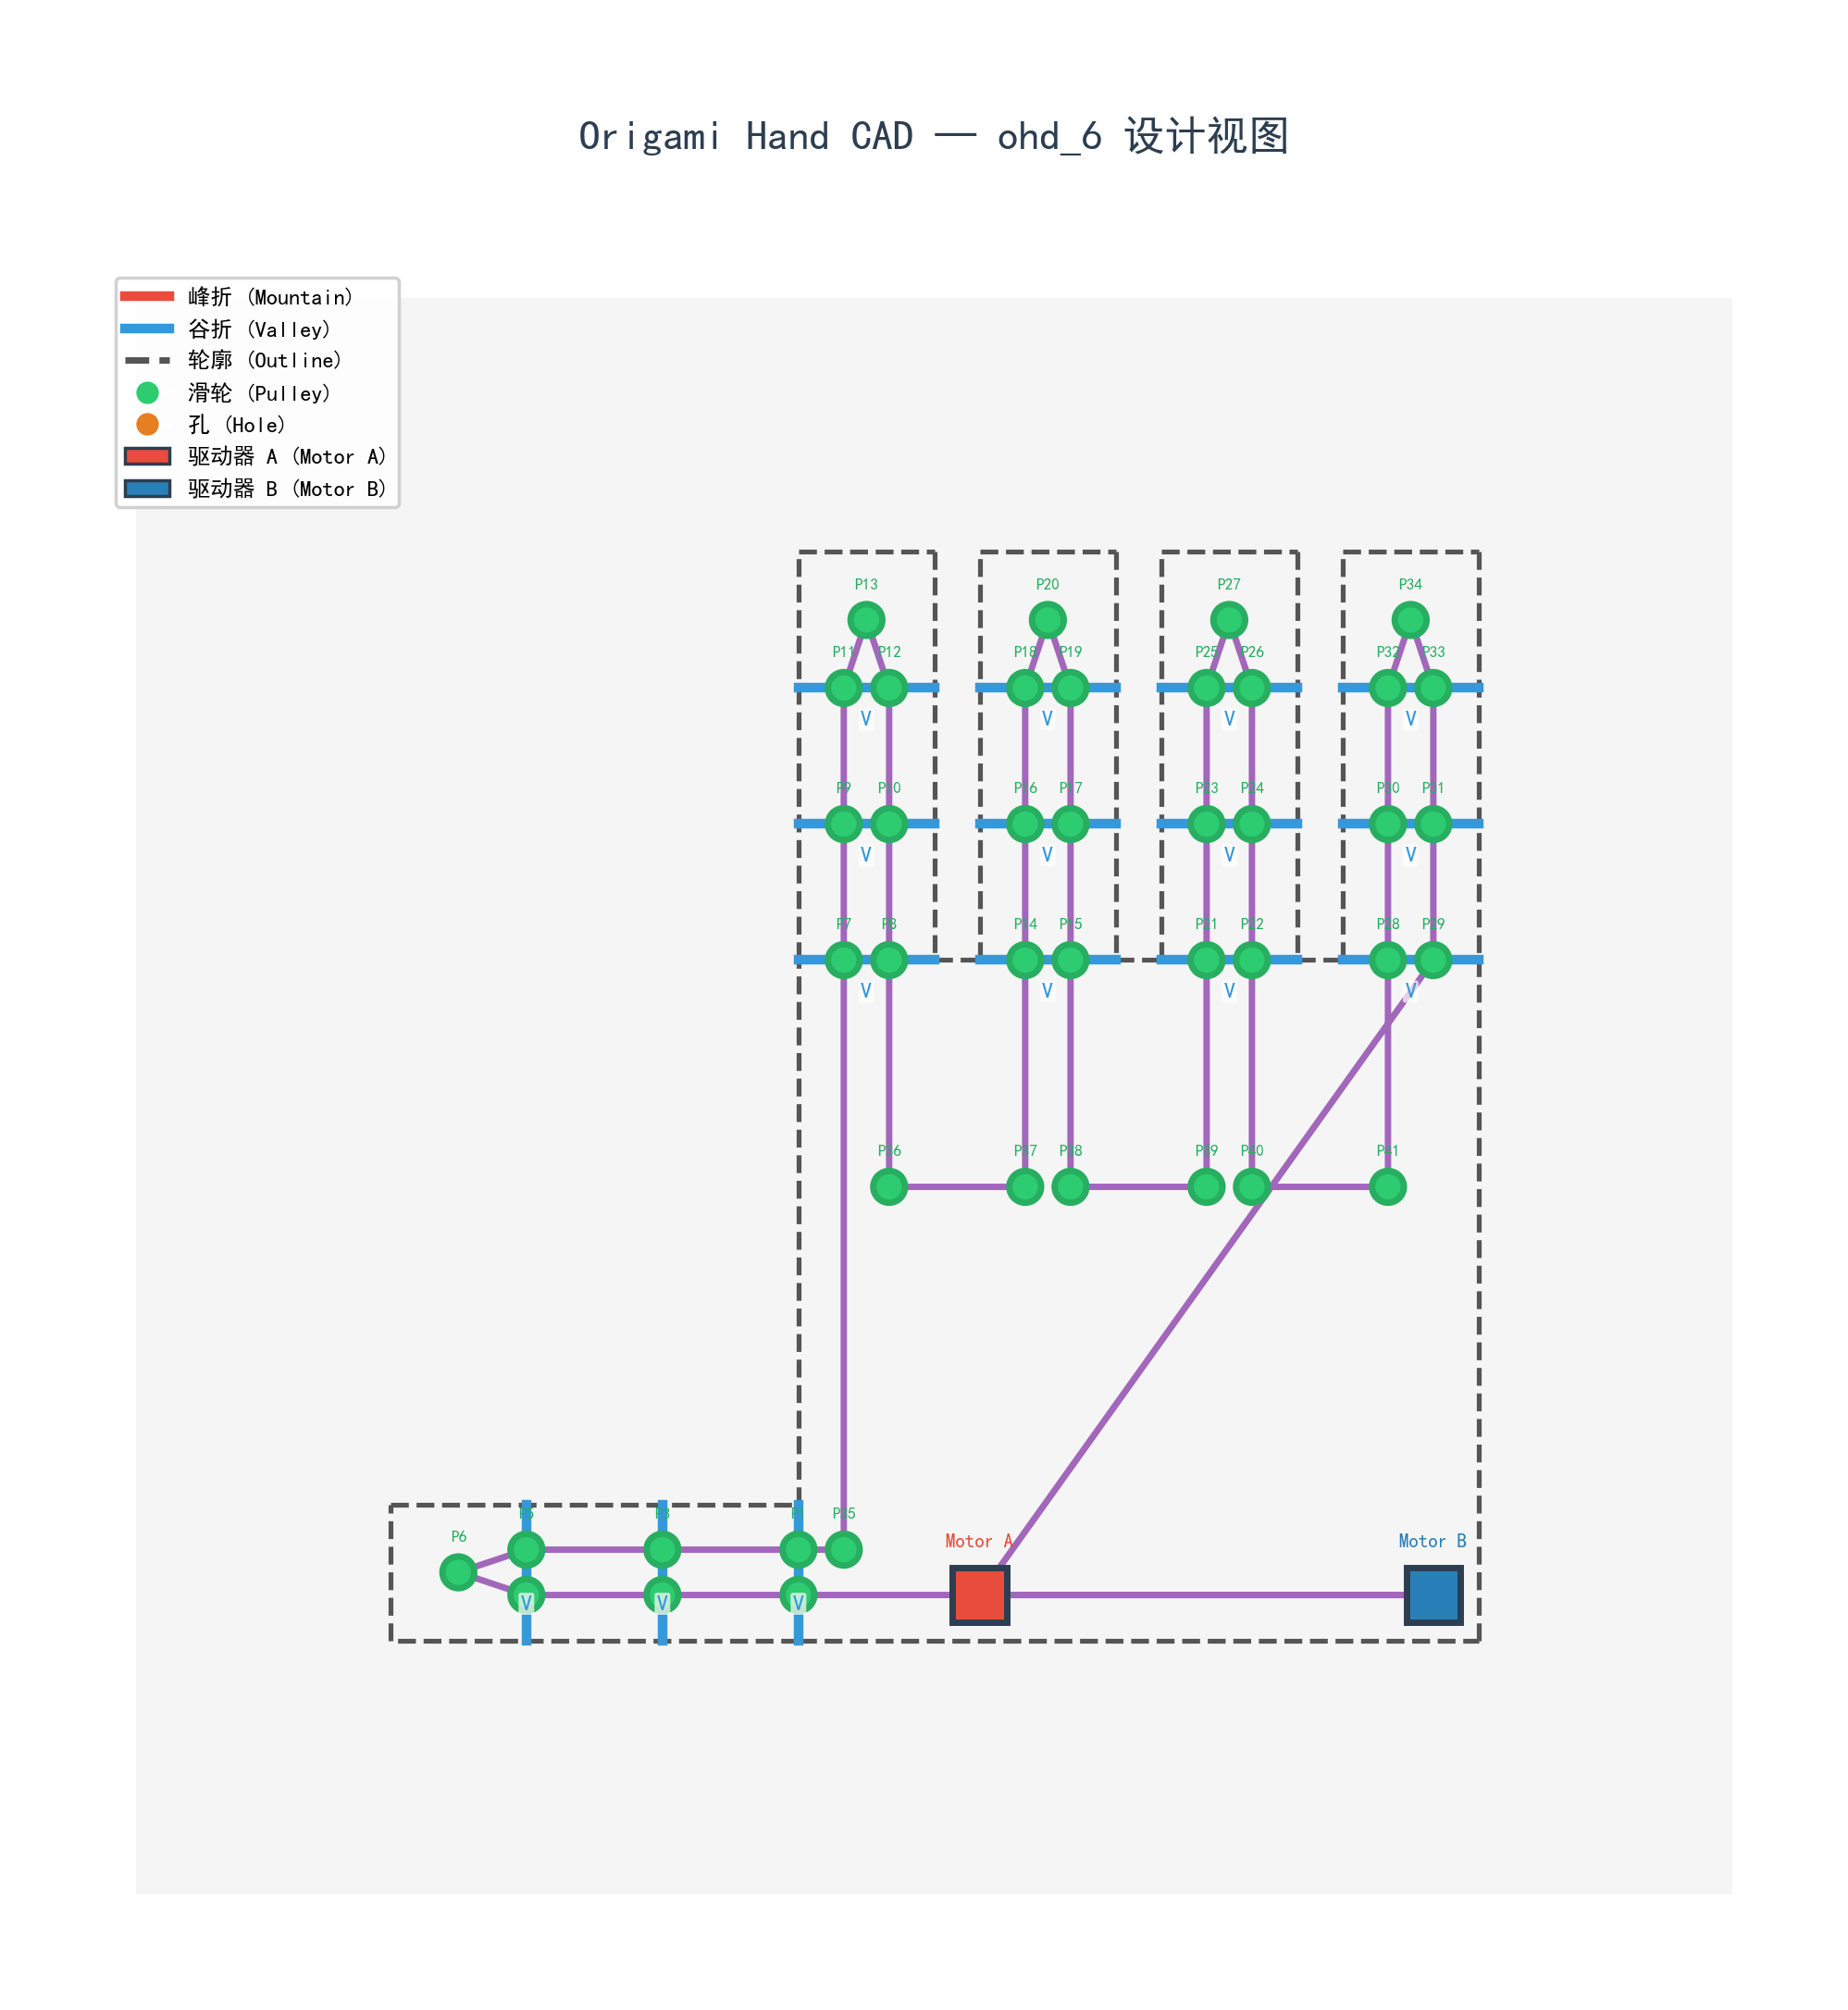
\includegraphics[width=0.82\linewidth]{figures/cad_ohd6_screenshot.png}}

{\small Fig. 1. The project represents an origami hand with faces, creases, joints, holes, actuators, and tendon routes.}
\end{center}

\posterblock{deepblue}{lightgreen}{Literature Review}
Rigid synergy compresses high-dimensional hand posture into a low-dimensional command. Soft synergy treats that command as a compliant reference rather than a rigid final shape. Adaptive synergy connects the idea to hardware through tendon or differential transmissions. The SDAS/FMAs model proposed here extends adaptive synergy to a two-ended closed-loop tendon.

\[
\textbf{Rigid:}\qquad q=S\sigma
\]

\[
\textbf{Soft:}\qquad q_r=S\sigma,\qquad J^T f_c=K(q_r-q)
\]

\[
\textbf{Adaptive:}\qquad Rq=x,\qquad
q=E^{-1}R^T(RE^{-1}R^T)^{-1}x
\]

\[
\textbf{SDAS/FMAs:}\qquad
R_A=A_A^T\bar{R},\quad R_B=A_B^T\bar{R}
\]

\[
\tau=R_A^T F_A+R_B^T F_B
\]

The key gap is the fixed-transmission assumption. A two-ended tendon needs two one-sided transmissions because the tension distribution depends on the pulling direction.

\columnbreak

\posterblock{deepblue}{lightorange}{Methodology}
The project has three connected layers. First, the design and geometric simulation layer parses \texttt{.ohd}/DXF data, builds topology, exports visual geometry, and maps low-dimensional commands to reference joint motion. Second, SDAS/FMAs derives a tendon-based synergy from two-ended closed-loop routing. Third, MuJoCo solves the resulting dynamics and contact constraints.

\[
\delta l=\bar{R}\delta q
\]

\[
T_j^{(A)}=\alpha_j^{(A)}F_A,\qquad
T_j^{(B)}=\alpha_j^{(B)}F_B
\]

\[
R_A=A_A^T\bar{R},\qquad R_B=A_B^T\bar{R}
\]

\[
q=S_Ax_A+S_Bx_B+CJ^Tf_c
\]

\[
\sigma=\frac{x_A+x_B}{2},\qquad
\sigma_f=\frac{x_A-x_B}{2}
\]

\[
q=(S_A+S_B)\sigma+(S_A-S_B)\sigma_f+CJ^Tf_c
\]

\[
M(q)\ddot{q}+h(q,\dot{q})
=\tau_{\mathrm{SDAS}}(t)+J_c(q)^T\lambda
\]

\begin{center}
\fbox{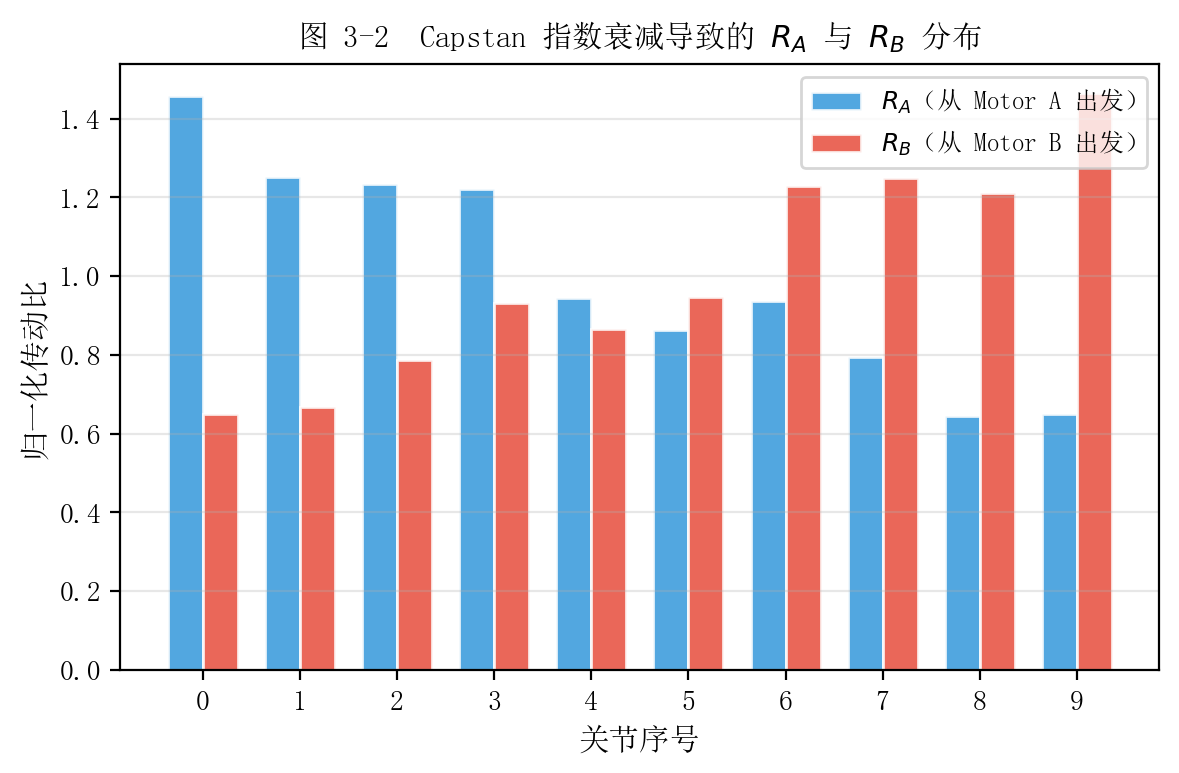
\includegraphics[width=0.76\linewidth]{figures/RA_RB_distribution.png}}

{\small Fig. 2. SDAS/FMAs separates the A-side and B-side tendon transmissions.}
\end{center}

\posterblock{deepblue}{lightpurple}{Experimental Results}
The results are selected to show the full project chain: design representation, reference motion, numerical state, and contact grasping. A free-space step input compares the geometric reference and the MuJoCo state. Contact scenes then show how SDAS/FMAs actuation behaves under object constraints.

\begin{center}
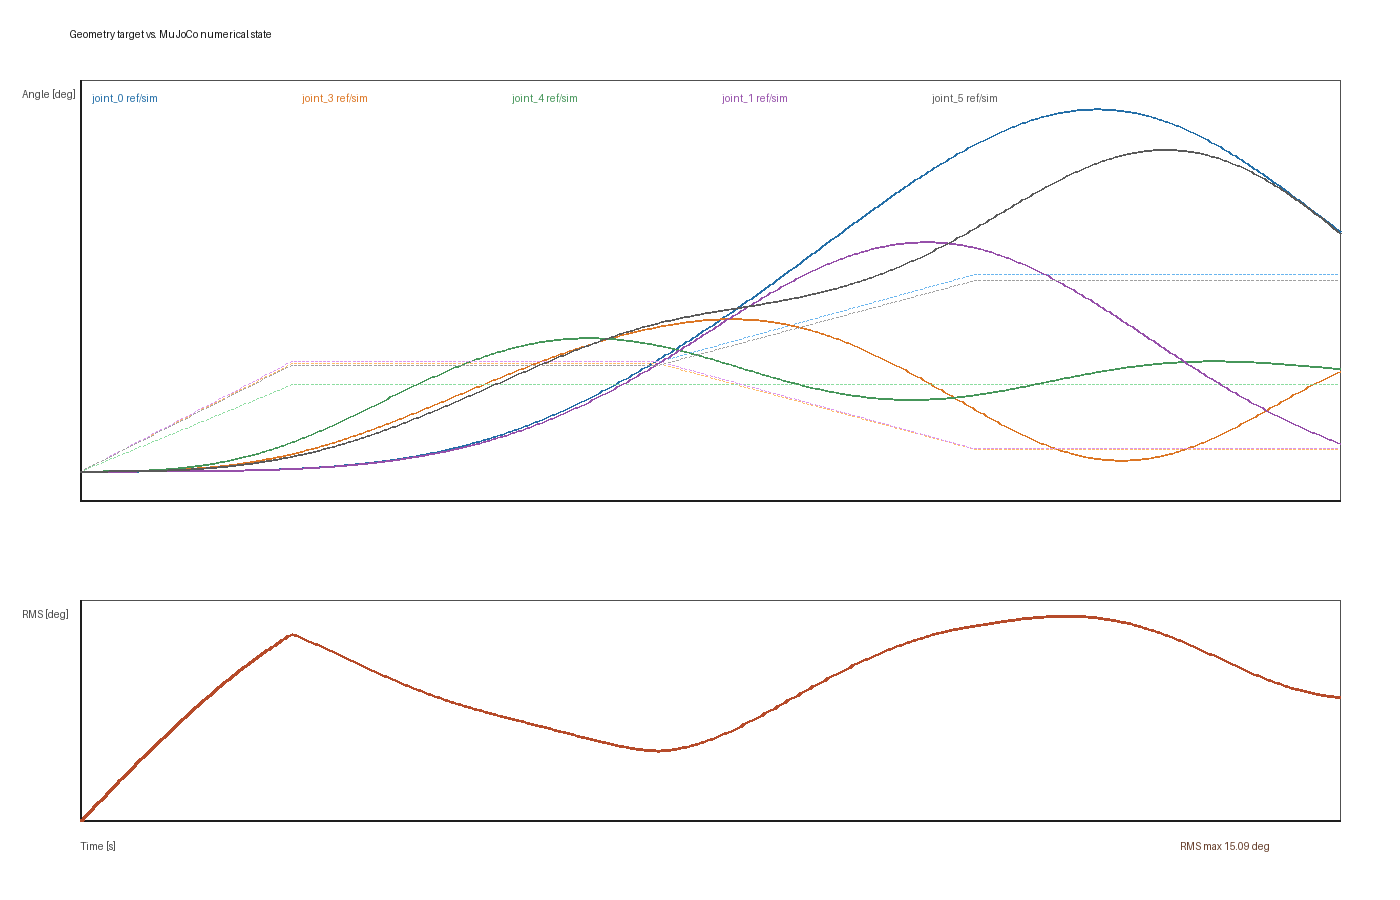
\includegraphics[width=0.92\linewidth]{../outputs/mujoco_sdas/step_demo/mujoco_sdas_step_geometry_vs_mujoco.png}

{\small Fig. 3. Geometry/SDAS reference versus MuJoCo numerical state.}
\end{center}

\columnbreak

\posterblock{deepblue}{lightpurple}{Representative Contact Demos}
\begin{center}
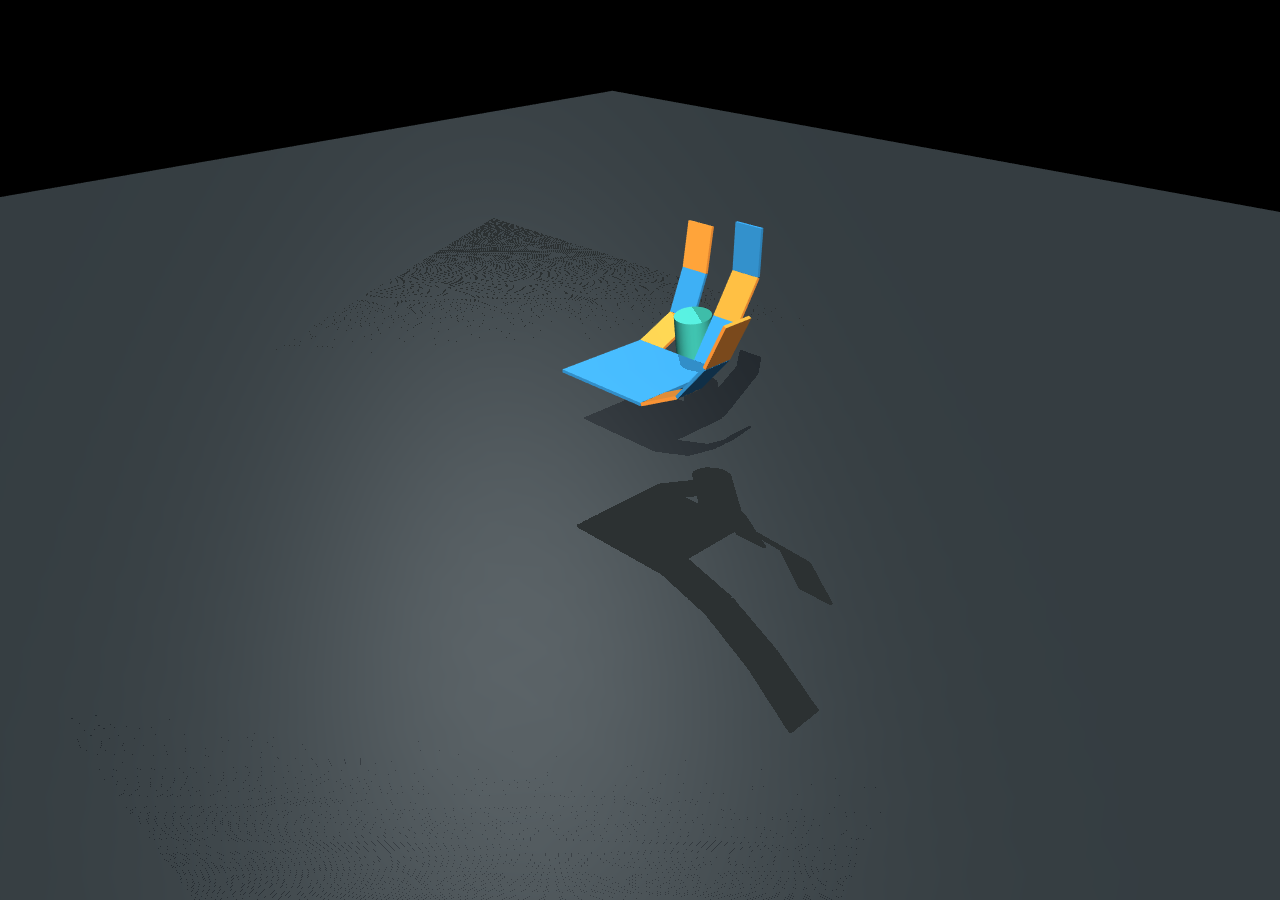
\includegraphics[width=0.48\linewidth]{../outputs/mujoco_sdas/grasp_cylinder/mujoco_sdas_grasp_cylinder_t1.250.png}
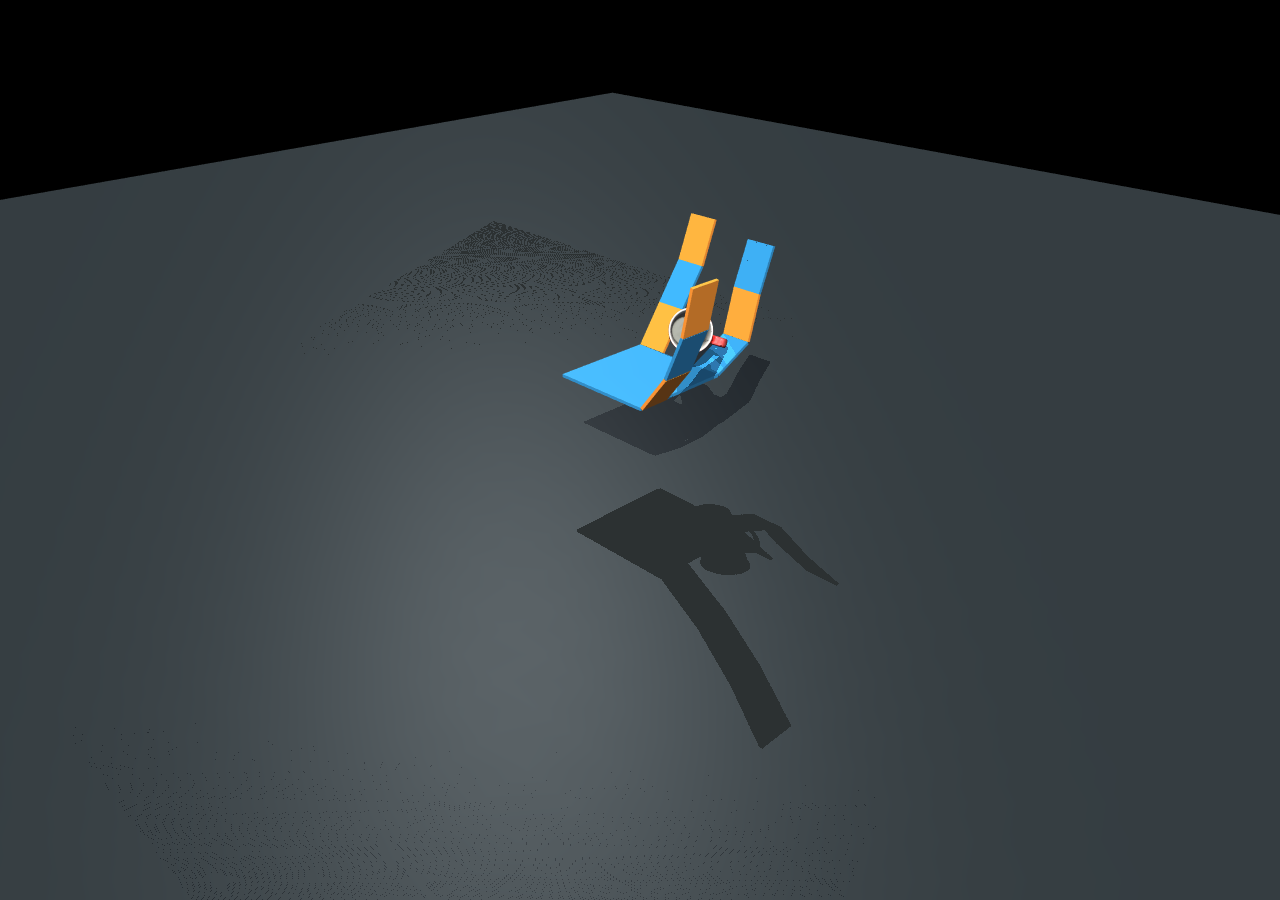
\includegraphics[width=0.48\linewidth]{../outputs/mujoco_sdas/grasp_scanned_mug/mujoco_sdas_grasp_scanned_mug_t1.250.png}

{\small Fig. 4. Cylinder and scanned-mug grasping demos.}
\end{center}

\vspace{0.3em}

\begin{center}
\small
\begin{tabular}{>{\raggedright\arraybackslash}p{0.27\linewidth}rrrr}
\toprule
Demo & Steps & Contact steps & Max contacts & RMS \\
\midrule
Free step & 600 & 0 & 0 & 0.1848 \\
Cylinder & 700 & 158 & 5 & 0.1816 \\
Scanned mug & 700 & 209 & 7 & 0.1821 \\
\bottomrule
\end{tabular}
\end{center}

\[
F_{\mathrm{contact,total}}(t)
=
\sum_{i=1}^{n_c(t)}\|f_{c,i}(t)\|
\]

\posterblock{deepblue}{lightblue}{Conclusion}
The contribution is a full modeling chain: origami hand design, geometric synergy simulation, SDAS/FMAs tendon transmission, and MuJoCo contact-aware numerical grasping. The project does not only render a final posture; it explains how the designed tendon routing produces a low-dimensional actuation model and how that model behaves under numerical dynamics and object contact.

\[
\texttt{.ohd design}
\rightarrow
q_{\mathrm{ref}}
\rightarrow
\tau_{\mathrm{SDAS}}
\rightarrow
\text{MuJoCo contact simulation}
\]

\vspace{0.4em}
{\small References: Santello et al. 1998; Bicchi et al. 2011; Catalano et al. 2014; Todorov et al. 2012.}

\end{multicols}

\end{document}
